%% 
%% Copyright 2019-2024 Elsevier Ltd
%% 
%% This file is part of the 'CAS Bundle'.
%% --------------------------------------
%% 
%% It may be distributed under the conditions of the LaTeX Project Public
%% License, either version 1.3c of this license or (at your option) any
%% later version.  The latest version of this license is in
%%    http://www.latex-project.org/lppl.txt
%% and version 1.3c or later is part of all distributions of LaTeX
%% version 1999/12/01 or later.
%% 
%% The list of all files belonging to the 'CAS Bundle' is
%% given in the file `manifest.txt'.
%% 
%% Template article for cas-dc documentclass for 
%% double column output.

\documentclass[a4paper,fleqn]{cas-dc}

% If the frontmatter runs over more than one page
% use the longmktitle option.

%\documentclass[a4paper,fleqn,longmktitle]{cas-dc}

%\usepackage[numbers]{natbib}
%\usepackage[authoryear]{natbib}
\usepackage[authoryear,longnamesfirst]{natbib}

%%%Author macros
\def\tsc#1{\csdef{#1}{\textsc{\lowercase{#1}}\xspace}}
\tsc{WGM}
\tsc{QE}
%%%

% Uncomment and use as if needed
%\newtheorem{theorem}{Theorem}
%\newtheorem{lemma}[theorem]{Lemma}
%\newdefinition{rmk}{Remark}
%\newproof{pf}{Proof}
%\newproof{pot}{Proof of Theorem \ref{thm}}

\begin{document}
\let\WriteBookmarks\relax
\def\floatpagepagefraction{1}
\def\textpagefraction{.001}

% Short title
\shorttitle{Bensemble Technical Report}    

% Short author
\shortauthors{Sobolevsky et al.}  

% Main title of the paper
\title [mode = title]{Bensemble: A Python Library for Bayesian Ensembling}  

% Title footnote mark
% eg: \tnotemark[1]
% \tnotemark[1] 

% Title footnote 1.
% eg: \tnotetext[1]{Title footnote text}
% \tnotetext[1]{} 

% First author
%
% Options: Use if required
% eg: \author[1,3]{Author Name}[type=editor,
%       style=chinese,
%       auid=000,
%       bioid=1,
%       prefix=Sir,
%       orcid=0000-0000-0000-0000,
%       facebook=<facebook id>,
%       twitter=<twitter id>,
%       linkedin=<linkedin id>,
%       gplus=<gplus id>]

\author[1,2]{Fedor Sobolevsky}%[<options>]

% Corresponding author indication
% \cormark[1]

% % Footnote of the first author
% \fnmark[1]

% % Email id of the first author
% \ead{}

% % URL of the first author
% \ead[url]{}

% % Credit authorship
% % eg: \credit{Conceptualization of this study, Methodology, Software}
% \credit{}

% Address/affiliation
\affiliation[1]{organization={Moscow Institute of Physics and Technology},
            % addressline={}, 
            city={Moscow},
%          citysep={}, % Uncomment if no comma needed between city and postcode
            % postcode={}, 
            % state={},
            country={Russia}}

\affiliation[2]{organization={Moscow State University},
            % addressline={}, 
            city={Moscow},
%          citysep={}, % Uncomment if no comma needed between city and postcode
            % postcode={}, 
            % state={},
            country={Russia}}

\author[1]{Dmitrii Vasilenko}%[]

\author[1]{Mukhammadsharif Nabiev}%[]

% % Footnote of the second author
% \fnmark[2]

% % Email id of the second author
% \ead{}

% % URL of the second author
% \ead[url]{}

% % Credit authorship
% \credit{}


\author[1]{Vadim Kasyuk}%[]


% Corresponding author text
% \cortext[1]{Corresponding author}

% Footnote text
% \fntext[1]{}

% For a title note without a number/mark
%\nonumnote{}

% Here goes the abstract
\begin{abstract}
    In this technical report, we introduce Bensemble, a Python library designed for approximating the posterior distribution of neural network weights to facilitate Bayesian ensembling. Standard deep learning models often yield overconfident predictions, since they typically don't take into account the uncertainty which comes with model training. Our library addresses this by providing a unified, PyTorch- and Lightning-compatible interface for a variety of Bayesian ensembling methods, including variational inference, probabilistic backpropagation, Laplace approximation, neural ensemble search and others. Bensemble operates on the principle that stochastic weight distributions act as generators for diverse model ensembles. It decouples the inference phase (learning an approximation of the posterior) from the prediction phase (sampling deterministic members for Bayesian model averaging). We provide a detailed description of Bensemble's interface and implemented methods. We also demonstrate the library's capabilities on benchmarks focusing on calibration and adversarial robustness.
\end{abstract}

% Use if graphical abstract is present
%\begin{graphicalabstract}
%\includegraphics{}
%\end{graphicalabstract}

% Research highlights
\begin{highlights}
\item A unified framework for Bayesian ensembling methods, PyTorch-compatible.
\item Diversity of implemented ensembling methods, including variational inference, probabilistic backpropagation, neural ensemble search and more.
\item Evaluated on several benchmarks to ensure functionality and compare implemented methods.
\end{highlights}


%\nocite{*}

% Keywords
% Each keyword is seperated by \sep
\begin{keywords}
Bayesian ensembling \sep uncertainty \sep PyTorch \sep Python
\end{keywords}

\maketitle


\section{Introduction}
Standard neural networks typically optimize a point estimate of their weights, which fails to capture epistemic uncertainty. Bayesian ensembling methods offer an alternative approach by approximating a probability distribution over model weights. This enables uncertainty estimation by averaging model predictions over the weight posterior. While exact inference is intractable, approximate methods allow us to learn a surrogate distribution over model weights. This approximated posterior can be treated as a source from which we sample an ensemble of deterministic models. Prediction and uncertainty estimation can then be done by aggregating predictions across this ensemble.  

Currently, there exists a wide variety of methods implementing different solutions to the problem of weight posterior approximation. These methods use different techniques and training/post-training procedure, and so far their implementations have been scattered across multiple interfaces and libraries. To solve this issue, we propose Bensemble, a library that implements a wide variety of Bayesian ensembling methods and standardizes the workflow of probabilistic deep learning.

Our work makes the following main contributions:
\begin{enumerate}
    \item We introduce Bensemble, a Python library with a unified API that abstracts the complexity of seven different Bayesian ensembling methods and their variations, allowing for standardized usage and convenient method comparison.
    \item We provide a variety of helper methods in Bensemble useful for probabilistic deep learning and model ensembling, as well as PyTorch and Lightning compatibility.
    \item We conduct extensive testing of all of Bensemble's methods to ensure quality implementations and provide sensible defaults for hyperparameters derived from testing.
\end{enumerate}

\begin{figure}
    \centering
    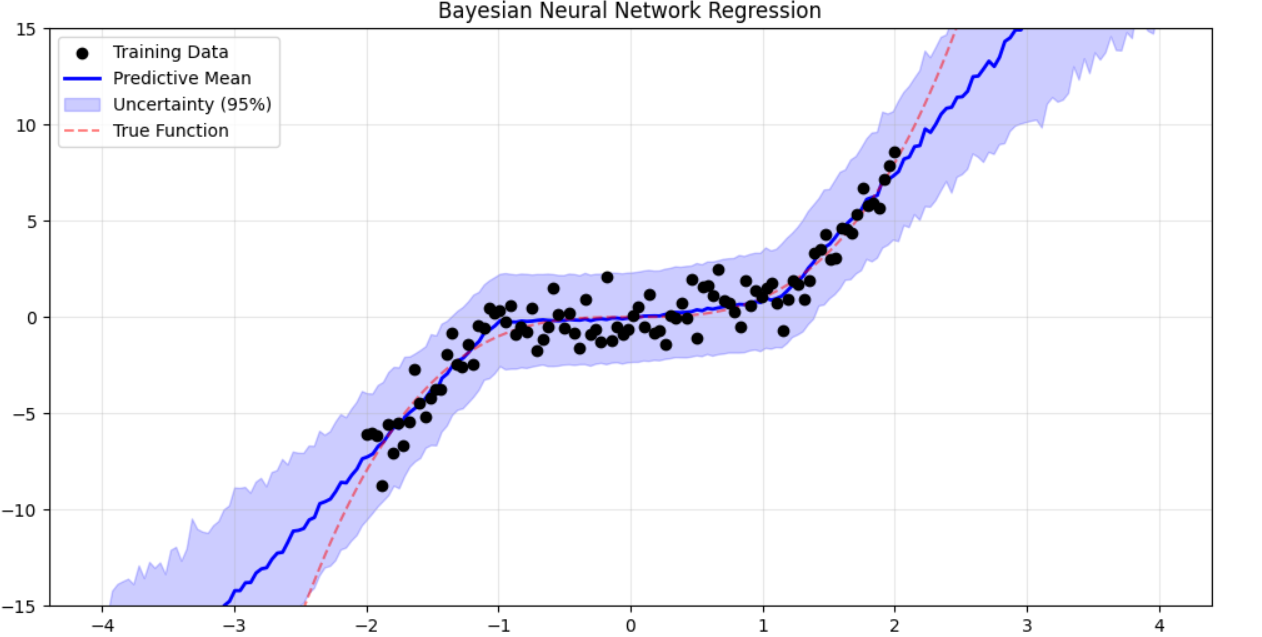
\includegraphics[width=\linewidth]{img/example.png}
    \caption{An example of regression with uncertainty using VI}
    \label{fig:example}
\end{figure}

\section{Methodology}

\subsection{Problem Statement}
Bensemble's core objective is weight posterior approximation for neural networks. Formally, given a dataset \(\mathcal{D}=\{(x_i,y_i)\}_{i=1}^N\) and a neural network with weights $w$, we seek the posterior distribution 
$$
p(w\mid\mathcal{D}) \propto p(\mathcal{D}\mid w)p(w).
$$
Since the exact posterior is intractable in the case of most neural networks, we apply a variety of different methods to approximate the true posterior with a parametric distribution $q_\theta(w)$. From this distribution, we can sample various sets of model weights to produce an ensemble of models $f_{w_i}$. Predictions are then made by averaging predictions of each member model from the ensemble:
$$
\hat{y} = \sum\limits_{i=1}^K f_{w_i}(x).
$$
Uncertainty of predictions can be then defined as the standard deviation of member predictions (see figure~\ref{fig:example}).

\subsection{Implemented methods}
We will now briefly describe the methods implemented as part of Bensemble.

Following \cite{gal2016dropout}, we implement \textbf{Monte-Carlo dropout (MCD)} as a Bayesian ensembling method. For a neural network trained with dropout, this method works by leaving dropout on at the inference stage. This way, we get an ensemble of models, each with random weight subsamples from the original model.

We adopt the \textbf{practical variational inference (PVI)} framework proposed by \cite{graves2011practical}, approximating the posterior with a diagonal Gaussian \(q_\theta(w)\). The objective is to minimize the variational free energy, often interpreted as a Minimum Description Length (MDL) cost:
$$
    \mathcal{L}(\theta) = \underbrace{\mathbb{E}_{q_\theta(w)}[\mathcal{L}_{\mathcal{D}}(w)]}_{\text{error cost}} + \underbrace{\mathrm{KL}(q_\theta(w) \| p(w))}_{\text{complexity cost}},
$$
where \(\mathcal{L}_{\mathcal{D}}\) is the negative log-likelihood.

To optimize the error cost efficiently, we employ the local reparameterization trick (LRT) \cite{kingma2015variational}. As noted by \cite{graves2011practical}, sampling weights directly introduces high variance in gradient estimates. LRT addresses this by sampling pre-activations instead. For a linear layer with inputs \(X\), weight means \(M\), and variances \(V\), the pre-activation \(\Gamma\) is distributed as:
$$
\Gamma \sim \mathcal{N}(XM^T, X^2 V^T).
$$\
We sample \(\zeta = XM^T + \varepsilon \odot \sqrt{X^2 V^T}\), where \(\varepsilon \sim \mathcal{N}(0, I)\), allowing for stable, low-variance backpropagation. The complexity cost is computed analytically as the sum of KL divergences for each weight.

For \textbf{variational inference with Rényi divergence (VR)}, introduced by \cite{li2016renyi}, we implement a weight perturbation approach. Unlike our VI implementation, here, explicit weights \(w \sim \mathcal{N}(\mu, \text{softplus}(\rho))\) are sampled during the forward pass. The objective generalizes the ELBO using \(\alpha\)-Rényi divergence:
$$
\mathcal{L}_{\text{VR}}(\theta, \alpha) = -\frac{1}{1-\alpha} \log \frac{1}{K} \sum_{k=1}^K \left( \frac{p(\mathcal{D}, w_k)}{q_\theta(w_k)} \right)^{1-\alpha}.
$$
The parameter \(\alpha\) (default 1.0) controls the bias-variance trade-off.

Our implementation of \textbf{probabilistic backpropagation (PBP)} by \cite{hernandez2015probabilistic} uses assumed density filtering (ADF) in an online fashion. Means and variances are propagated analytically. For ReLU activations, we use exact moment matching functions relying on the PDF/CDF of the standard normal. Weights are updated by matching the moments of the tilted distribution \(q(w)p(y|x,w)\). We compute gradients of the log-partition function \(\log Z\) to update \(\mu\) and \(\Sigma\) directly, bypassing standard SGD.

We also implement a scalable \textbf{Laplace approximation (LA)} using Kronecker-factored approximate curvature as described in \cite{ritter2018scalable}. Since this is, unlike others, a post-hoc posterior approximation method, a standard network is first trained to find the mode \(W^{\text{MAP}}_l\). We then capture covariance of activations ($A_{l}$) and pre-activation gradients ($G_l$). The posterior for layer $l$ is then approximated as a matrix normal distribution \(\mathcal{MN}(W^{\text{MAP}}_l, A_l, G_l)\). Samples are generated efficiently using eigen-decomposition of Kronecker factors:
\begin{equation}
    W_{\text{sample}} = W_{\text{MAP}} + L_V Z L_U^T,
\end{equation}
where $L_V, L_U$ are Cholesky factors of the inverse regularized covariances and $Z$ is sampled from the standard matrix normal distribution.

\textbf{Neural ensemble search (NES)}, introduced by \cite{zaidi2021neural}, employs neural architecture search in order to find an optimal ensemble of models with varying architectures. Formally, the method searches through model architectures $\alpha_i$ in a predefined architecture search space $\mathcal{A}$. To find the optimal ensemble, NES solves the following bilevel optimization problem:
$$
\min_{\alpha_1, \dots, \alpha_M \in \mathcal{A}} \mathcal{L}\!\left(\mathrm{Ensemble}(f_{\theta_1,\alpha_1}, \dots, f_{\theta_M,\alpha_M}),\, \mathcal{D}_{\mathrm{val}}\right)
$$$$
\text{s.t.} \quad \theta_i \in \operatorname*{arg\,min}_{\theta}\, \mathcal{L}(f_{\theta,\alpha_i}, \mathcal{D}_{\mathrm{train}}), \quad i = 1, \dots, M
$$
For architecture searching, we implement both strategies described in \cite{zaidi2021neural}~--- random searching (NES-RS) and regularized evolution (NES-RE). While the first strategy relies on a simple random searching procedure, the second one utilizes an evolutionary algorithm.

Finally, we also implement \textbf{neural ensemble search via Bayesian sampling (NESBS)}, introduced by \cite{shu2022neural}, as an alternative to NES that aims to reduce the computational cost of NES. To do so, it utilizes training a supernet with uniform path sampling to share weights across different model architectures. Then, a variational posterior over architectures is introduced:
$$
p_{\alpha}(\mathcal{A})\approx p(\mathcal{A} | \mathcal{D}).
$$
The variational posterior is learned via evidence lower bound (ELBO) minimization: 
$$
\max_\alpha \mathbb{E}_{\mathcal{A}\sim p_{\alpha}(\mathcal{A})} [\log p(\mathcal{A}|\mathcal{D})] - KL[p_{\alpha}(\mathcal{A})|p(\mathcal{A})].
$$
Ensemble member architectures can then be sampled from the variational posterior via simple Monte-Carlo sampling or using Stein variational gradient descent with regularized diversity (SVGD-RD), i.\,e. via controlled optimization of the set of architectures with the following objective:
$$
q^* = \arg\min_{q\in\mathcal{Q}} \text{KL}(q\|p) + n\delta\mathbb{E}_{x, x' \sim q}[k(x, x')].
$$

\section{Implementation Details}
The architecture of Bensemble is built around the `Ensemble` class, incapsulating an ensemble of models or a stochastic ensemble (i.\e. an ensemble where model weights are sampled in an online fashion). Each of Bensemble's methods can be used to produce an instance of this base class, which then can be used to make predictions with uncertainty.

MCD, VR, VI and PBP are all implemented as stochastic ensemble generators. Notably, while we implement most of the methods as self-contained classes, VI is implemented via a Bayesian linear layer class. LA and NES variants are implemented as generators of model ensembles. We implement neural ensemble search algorithm via integration with the NNI library \cite{Microsoft_Neural_Network_Intelligence_2021}.

We also implement a variety of utilities for Bayesian machine learning in Bensemble, including but not limited to: uncertainty decomposition (into aleatoric and epistemic components), evaluation metrics (NLL, ECE, Brier score) and calibration for classification probabilities (temperature scaling and vector scaling). The library's full code is available at \texttt{github.com/intsystems/bensemble}.


\section{Experimental Evaluation}

\subsection{Experimental setup}
We evaluated the library on the Boston Housing dataset \cite{harrison1978hedonic}, as well as synthetic classification and regression datasets. The methods were applied to an MLP with a fixed architecture made of two hidden layers with size 50 and ReLU activations. MCD was used with adropout rate of 0.2. For PBP, we use an inverse Gamma prior with noise shape parameters $\alpha=6.0, \beta=6.0$. For Laplace, we perform MAP training with learning rate $\alpha=10^{-3}$ and K-FAC estimated on the full training set. VI and VR were tested with priors with $\sigma=1.0$, initialized by $\rho=-2.0$ (approximately $\sigma=0.12$). For NES, we used a simple search space with varying hidden layer counts, sizes and varying dropout rates. NESBS was used with temperature 0.8, 8 SVGD steps and a learning rate of 0.25 for SVGD.

\subsection{Synthetic data}
\begin{figure*}[ht]
    \centering
    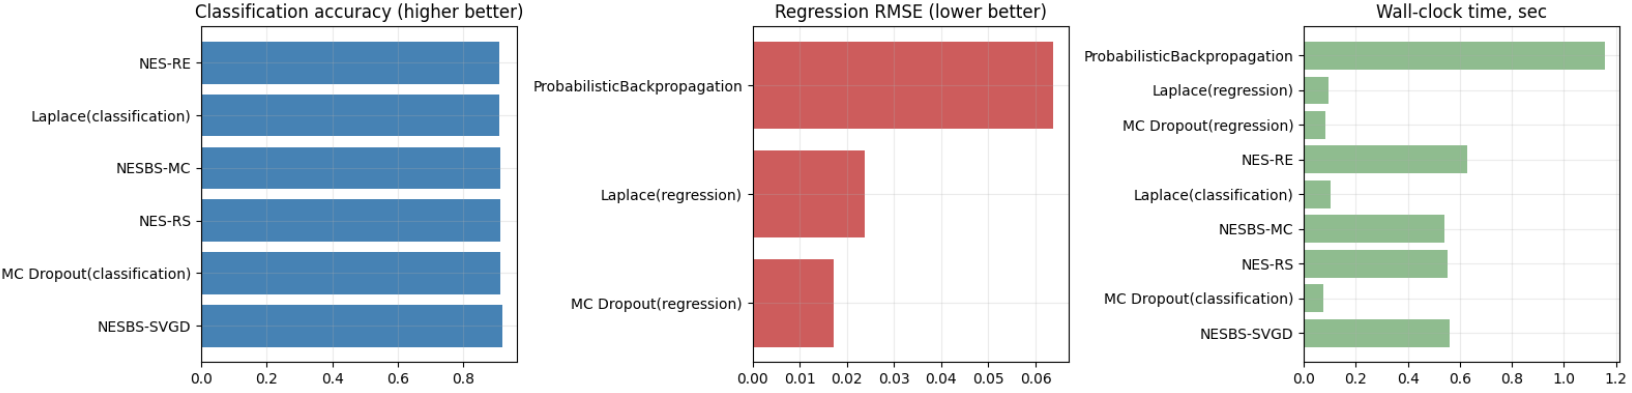
\includegraphics[width=\textwidth]{img/benchmark_results.png}
    \caption{Results on synthetic dataset}
    \label{fig:benchmark_results}
\end{figure*}

Figure~\ref{fig:benchmark_results} presents the results of evaluation on synthetic classification and regression datasets. We can see that, overall, all methods perform well, with some exceeding others in accuracy and some leading in time performance.

\subsection{Boston Housing dataset}
Table \ref{tab:boston_results} shows the results of evaluation on the Boston Housing dataset. We can see that while deterministic models are accurate (low RMSE), they are poorly calibrated (high NLL). PBP and VI achieve the best balance of accuracy and calibration.

\begin{table}[ht]
\centering
\caption{Performance on Boston Housing (Test Set). Lower is better.}
\label{tab:boston_results}
\begin{tabular}{lcccc}
\toprule
\textbf{Method} & \textbf{RMSE} & \textbf{NLL} & \textbf{ECE} & \textbf{Brier} \\
\midrule
Deterministic MLP & 4.21 & 47.99 & 0.033 & 0.090 \\
MCD & \textbf{3.84} & 3.68 & 0.019 & \textbf{0.055} \\
VI & 4.63 & \textbf{2.88} & 0.008 & 0.099 \\
PBP & 5.42 & 3.17 & 0.008 & 0.091 \\
VR & 5.36 & 3.16 & \textbf{0.006} & 0.127 \\
LA & 19.38 & 4.55 & 0.011 & 0.241 \\
\bottomrule
\end{tabular}
\end{table}

\subsection{Adversarial Robustness}
\begin{table}[ht]
\centering
\caption{RMSE under FGSM adversarial attacks. \textbf{Bold} indicates best performance.}
\label{tab:adversarial_rmse}
\begin{tabular}{lcccccc}
\toprule
Method & 0.00 & 0.10 & 0.30 & 0.50 & 1.00 \\
\midrule
Det. MLP & 4.21 & 7.41 & 13.13 & 17.70 & 27.74 \\
MCD & \textbf{3.80} & \textbf{5.16} & 8.82 & 12.67 & 23.05 \\
VI & 4.58 & \textbf{5.16} & \textbf{6.40} & \textbf{7.71} & \textbf{12.22} \\
PBP & 5.42 & 5.73 & 6.87 & 8.28 & 12.34 \\
VR & 5.35 & 5.76 & 6.64 & 8.74 & 13.50 \\
LA & 19.22 & 24.04 & 22.92 & 26.40 & 40.46 \\
\bottomrule
\end{tabular}
\end{table}

We subjected models to FGSM attacks (Table \ref{tab:adversarial_rmse}). The deterministic model fails catastrophically at $\varepsilon=0.1$. VI and PBP demonstrate superior robustness. Specifically, PBP's moment matching effectively filters high-frequency adversarial noise, maintaining low error rates even at high perturbation levels.

\section{Conclusion}
We presented Bensemble, a library that democratizes access to stochastic weight modeling. We implemented a wide variety of Bayesian ensembling methods, applicable to different tasks and in various usage scenarios. By validating our implementations of these methods on a number of benchmarks, we ensure that Bensemble provides a robust toolkit for uncertainty estimation. Our experiments confirm that Bayesian ensembling noticeably improves calibration and adversarial robustness compared to standard point estimates.

% Main text
% \section{}\label{}

% Numbered list
% Use the style of numbering in square brackets.
% If nothing is used, default style will be taken.
%\begin{enumerate}[a)]
%\item 
%\item 
%\item 
%\end{enumerate}  

% Unnumbered list
%\begin{itemize}
%\item 
%\item 
%\item 
%\end{itemize}  

% Description list
%\begin{description}
%\item[]
%\item[] 
%\item[] 
%\end{description}  

% \clearpage %%Remove this from your manuscript

% Figure
% \begin{figure}%[]
%   \centering
% %    \includegraphics{}
%     \caption{}\label{fig1}
% \end{figure}


% \begin{table}%[]
% \caption{}\label{tbl1}
% \begin{tabular*}{\tblwidth}{@{}LL@{}}
% \toprule
%   &  \\ % Table header row
% \midrule
%  & \\
%  & \\
%  & \\
%  & \\
% \bottomrule
% \end{tabular*}
% \end{table}

% Uncomment and use as the case may be
%\begin{theorem} 
%\end{theorem}

% Uncomment and use as the case may be
%\begin{lemma} 
%\end{lemma}

%% The Appendices part is started with the command \appendix;
%% appendix sections are then done as normal sections
%% \appendix

% \section{}\label{}

% To print the credit authorship contribution details
\printcredits

%% Loading bibliography style file
%\bibliographystyle{model1-num-names}
\bibliographystyle{cas-model2-names}

% Loading bibliography database
\bibliography{cas-refs}

% Biography
%\bio{}
% Here goes the biography details.
%\endbio

%\bio{pic1}
% Here goes the biography details.
%\endbio

\end{document}

